\chapter{Materiali e Metodi}
%\`E

Questo lavoro di tesi è basato su uno studio osservazionale prospettico condotto presso l'ospedale universitario di terzo livello, istituto materno infantile --- IRCSS Burlo Garofolo di Trieste. In tale analisi si esamina il livello di soddisfazione percepito dal personale infermieristico in merito alla qualità della sedazione pediatrica al di fuori della sala operatoria, mettendo a confronto quattro agenti sedativi ed analgesici tra i più ampiamente utilizzati: propofol, midazolam, ketamina e dexmedetomidina. 
\\Dal momento che in letteratura non esiste uno strumento validato per la valutazione della percezione infermieristica, è stato formulato da un gruppo di pediatri, anestesisti pediatrici ed infermieri pediatrici un questionario appositamente designato agli scopi di questo studio. Dopo essere stato testato su un campione ridotto di 30 soggetti ed essere stato rifinito e corretto sulla base delle raccomandazioni fornite da questi primi partecipanti, è stato infine sottoposto a 51 infermieri esperti nel campo della sedazione peri-procedurale.

\section{Scelta dell'infermiere come indicatore di qualità}

La scelta di valutare la percezione del personale infermieristico deriva dalla necessità di ampliare ed oggettivare i risultati emersi nello studio riguardante la soddisfazione parentale, ampiamente descritto poco sopra \cite{Cortellazzo2022}. Infatti, mentre il caregiver viene facilmente influenzato da diversi fattori associati alla totalità del vissuto ospedaliero, dal servizio di parcheggio, alla simpatia del personale, finanche alla comparsa di complicanze correlate specificamente alla procedura; l'infermiere, in quanto figura professionale che assiste i pazienti durante tutte le fasi della procedura: dall'ammissione, al posizionamento dell'accesso venoso, al monitoraggio dei parametri vitali e alla somministrazione dei farmaci prima e durante la sedazione, fino poi al completo risveglio ed alla dimissione, risulta il candidato più adatto a giudicare in maniera oggettiva gli elementi associati alla sedazione ed al risveglio post procedurale. Inoltre, mentre il genitore esprime il proprio parere basandosi su un'unica o su limitate esperienze di analgosedazione, l'infermiere partecipa a molteplici sedazioni procedurali ogni mese ed è quindi in grado di confrontare diversi regimi farmacologici ed esprimere un giudizio complessivo basato sull'efficacia della sedazione, sulla facilità e sulla sicurezza della via di somministrazione, oltre che sull'incidenza media e la severità degli effetti avversi associati.
\\In conclusione, l'opinione dell'infermiere riveste un ruolo chiave non solo al fine di ottenere delle indicazioni utili per la scelta farmacologica ma anche come occasione per integrare le conoscenze mediche alle osservazioni di una figura di riferimento fondamentale per il paziente e la famiglia, quale quella dell'infermiere. La collaborazione tra la professionalità medica ed infermieristica rappresenta il presupposto migliore per garantire alla comunità una sempre maggiore attenzione alla qualità di cura. 

%in maniera risulta un candidato più adatto a giudicare in modo oggettivo  Inoltre, 
%Dalle conclusioni dello studio sopra descritto sulla soddisfazione parentale in merito alla sedazione procedurale pediatrica \cite{Cortellazzo2022}, è emersa la necessità di estendere l'analisi ad una figura professionale che possa confrontare fornire un giudizio oggettivo. Infatti, il caregiver può essere influenzato nella valutazione finale dall'esperienza medico ospedaliera vissuta nella sua interezza, che può includere alcune variabili non strettamente associate alla sedazione in sé, quali ad esempio la facilità di parcheggiare, la simpatia del personale, il coinvolgimento nel processo decisionale ed eventuali problematiche specificamente collegate alla procedura. Inoltre, esprime la propria opinione sulla base, nella maggior parte dei casi, di un'unica o di limitate esperienze di analgosedazione e possiede, quindi, scarse o nulle conoscenze rispetto ai regimi farmacologici alternativi. 
%La scelta dell'infermiere come indicatore di qualità della sedazione procedurale ha il compito sia di rispondere all'esigenza di ottenere dei risultati basati su un giudizio più oggettivo, sia di rappresentare un'opportunità di migliorare lo standard di cure e la qualità del risveglio post sedazione. Gli infermieri arruolati in questo lavoro di tesi sono tutti professionisti esperti nel campo della sedazione peri-procedurale, prendono parte mensilmente ad un numero variabile di procedure attuate con regimi farmacologici differenti, assistendo il paziente nelle fasi che precedono e seguono la procedura, fino al completo risveglio ed alla dimissione; inoltre posizionano i cateteri venosi periferici e cooperano con il medico durante la sedazione somministrando i farmaci e monitorando i parametri vitali del bambino. Concludendo, l'infermiere risulta il candidato più adatto a comparare i diversi regimi sedativi e può rappresentare la chiave di volta nel fornire delle indicazioni imparziali, che possano essere utili al sedatore per la scelta farmacologica. Inoltre, questa analisi pone le basi per un potenziare la collaborazione tra medico ed infermiere e garantire al paziente ed alla famiglia una sempre maggiore attenzione alla qualità di cura.

%al fine di migliorare lo standard di cure e la qualità del risveglio post sedazione
%A tale proposito l'infermiere potrebbe essere il candidato più adatto,
%circa la scelta del genitore come indicatore di qualità del servizio sanitario offerto in merito alla sedazione procedurale,
%, invece, potrebbe rispondere all'esigenza di oggettivare la percezione 
%che, comprendendo il giudizio infermieristico, permette di approfondire il rapporto medico-infermiere,

%l'analisi della sua percezione

\section{Questionario}

L'indagine è stata svolta in modo anonimo tramite una piattaforma web di Google e gli infermieri idonei sono stati invitati a partecipare per mezzo di un link inviato al loro indirizzo mail istituzionale. Previo consenso di adesione allo studio, è stato chiesto loro di completare un questionario, consistente in 13 domande a risposta multipla e 2 a risposta aperta. Alcune domande prevedevano più di una risposta possibile e i partecipanti avevano la possibilità di rispondere a tutti o solo ad alcuni quesiti. 
\\L'intervista ha preso in considerazione sia il profilo dell'infermiere in termini di esperienza lavorativa nel campo delle sedazioni procedurali, sia il suo livello di soddisfazione associato all'utilizzo di propofol, midazolam, ketamina, dexmedetomidina o delle loro combinazioni. Inoltre, sono stati testati la frequenza di osservazione dei principali effetti collaterali descritti in letteratura per tali agenti farmacologici, il profilo di sicurezza percepito, oltre che l'eventuale necessità di somministrare farmaci \emph{rescue} al risveglio. Infine, sono state valutate l'utilità dell'approccio non farmacologico e le preferenze in merito alle diverse vie di somministrazione possibili. 

\newpage

\begin{survey}[Questionario sulla sedazione per infermieri/e]{xkcdGreyishTeal}

%Cari tutti, stiamo somministrando un questionario per testare la vostra soddisfazione in tema di sedazione peri procedurale. Il tempo necessario per completarlo è 5 minuti. 
%Grazie a tutti per la collaborazione.

% xkcdLightGreyGreen xkcdGreyishTeal xkcdPaleTeal xkcdSteel xkcdPowderBlue xkcdSteelBlue xkcdLightBlueGrey
    
       \Query In quale reparto lavori? 
       \Qlines{1}
       
       \Query Quanti anni di esperienza hai nel campo delle sedazioni peri-procedurali in età pediatrica? 
       \Qlines{1}
       
       
       \Query Nel reparto in cui lavori, a quante sedazioni/risvegli assisti ogni mese?
       \begin{Qlist}
           \item < 10
           \item 10-20
           \item 21-30
           \item > 30
       \end{Qlist}
       

       \Query Come giudichi la qualità globale della sedazione per ognuno dei seguenti farmaci? (\emph{0:~per niente soddisfatto, 10: massima soddisfazione possibile})
       
       propofol : \hfill \Qrating{11} 
    
       ketamina : \hfill \Qrating{11}
    
        dexmedetomidina : \hfill \Qrating{11}
    
        midazolam : \hfill \Qrating{11}
    
       \Query Spesso per ottimizzare la sedazione, vengono utilizzate combinazioni dei farmaci soprariportati. Quanto l'utilizzo di più farmaci contemporaneamente influenza la tua soddisfazione?
       \begin{Qlist}
           \item per niente
           \item poco
           \item abbastanza
           \item molto
       \end{Qlist}
       
       \hfill continua...
       
       \newpage
       
       \Query Quali effetti collaterali riscontri maggiormente dopo la sedazione con ognuno dei seguenti farmaci? Più di una risposta è possibile. (\emph{0: sonnolenza, 1: irritabilità, 2: iperattività/irrequietezza, 3: allucinazioni, 4: incoordinazione/impaccio motorio, 5: cefalea, 6: vertigini, 7: alterazioni dell’appetito, 8: nausea/vomito, 9: dispnea, 10: altro}). 
    
           propofol : \hfill \Qrating{11} 
           
           ketamina : \hfill \Qrating{11} 
           
           dexmedetomidina : \hfill \Qrating{11} 
           
           midazolam : \hfill \Qrating{11} 
    
       \Query Quanto i seguenti effetti collaterali riducono la tua soddisfazione in merito alla sedazione peri procedurale? (\emph{0: per niente, 1: poco, 2: abbastanza, 3: molto}).
       
           sonnolenza: \hfill \Qrating{4} 
           
           
           irritabilità:  \hfill \Qrating{4}
           
           iperattività/irrequietezza: \hfill \Qrating{4}
           
           allucinazioni: \hfill \Qrating{4}
           
           incoordinazione/impaccio motorio: \hfill \Qrating{4}
           
           cefalea: \hfill \Qrating{4}
           
           vertigini: \hfill \Qrating{4}
           
           alterazioni dell’appetito: \hfill \Qrating{4}
           
           nausea/vomito: \hfill \Qrating{4}
           
           distress respiratorio: \hfill \Qrating{4}
    
       \Query Per quali di queste sedazioni è spesso necessario somministrare al risveglio un farmaco \emph{rescue} o sintomatico (ad esempio antiemetico)? Più di una risposta è possibile.
       \begin{Qlist}
           \item propofol 
           \item ketamina 
           \item dexmedetomidina 
           \item midazolam 
       \end{Qlist}
       
      \hfill continua...
       
       \newpage
       
       \Query In termini di sicurezza, quanto ti senti sicuro durante la sedazione con i seguenti farmaci (\emph{0: per niente, 1: poco, 2: molto})?
       
           propofol: \hfill \Qrating{3}
           
           ketamina: \hfill \Qrating{3}
           
           dexmedetomidina: \hfill \Qrating{3}
           
           midazolam: \hfill \Qrating{3}
    
       \bigskip 
       Se non ti senti sicuro, specifica il perché:
       \Qlines{2}
       
       \Query Ritieni preferibile una sedazione eseguita per via:
       \begin{Qlist}
           \item intranasale
           \item orale + intranasale
           \item intramuscolare
           \item endovenosa
       \end{Qlist}
       
       \bigskip
       
       Con quale farmaco? 
       \begin{Qlist}
            \item propofol
            \item ketamina
            \item dexmedetomidina
            \item midazolam
       \end{Qlist}
%\newpage

       %\Query Con quale farmaco?
        %\begin{Qlist}
           %\item propofol 
           %\item ketamina 
           %\item dexmedetomidina 
           %\item midazolam 
       %\end{Qlist}
       

       \Query Quanto ritieni utile l’utilizzo di tecniche di distrazione nei bambini per l’esecuzione di procedure non dolorose/minimamente dolorose (posizionamento dell'accesso venoso periferico, prelievo ematico, rimozione punti di sutura, ...)?
       \begin{Qlist}
           \item per niente
           \item abbastanza
           \item molto
           \item moltissimo
       \end{Qlist}
       
       \hfill continua...
       
       \newpage
       
       \Query Indipendentemente dal tipo di sedazione, preferiresti avere a disposizione un accesso venoso periferico?
       \begin{Qlist}
           \item mai
           \item sempre se il bambino è fragile (se è affetto ad esempio da sindromi genetiche, autismo, ritardo psico-motorio, ...)
           \item sempre
       \end{Qlist}
       
       \Query Indicate quali fra i seguenti aspetti della sedazione influenzano maggiormente la tua soddisfazione:
       \begin{Qlist}
            \item tipo di farmaco e via di somministrazione
            \item effetti collaterali durante la sedazione
            \item effetti collaterali dopo la sedazione
            \item qualità del risveglio
            \item tempi di risveglio
            \item necessità di utilizzare farmaci \emph{rescue}
            \item impegno infermieristico
            \item soddisfazione dei genitori
            \item soddisfazione del bambino
            \item altro: \Qline{6cm}
       \end{Qlist}
       
       \Query Cosa cambieresti rispetto agli standard attuali sul tipo di analgosedazione in età pediatrica nella tua Unità Operativa? 
       \Qlines{5}
       
       \Query Come vorresti che venisse sedato tuo figlio/a? \Qlines{3}
       
       \bigskip
       
\end{survey}

\section{Analisi Statistica}

Le analisi statistiche e le rappresentazioni grafiche sono state realizzate utilizzando la piattaforma \textsc{Matlab}\textsuperscript{\tiny\sffamily\textregistered}\!\,v9.9, complementata dallo \textsc{Statistics and Machine Learning Toolbox} v12.0. I dati sono stati statisticamente descritti sia come numeri, percentuali, mediane con incluse le differenze interquartile, sia con classiche raffigurazioni grafiche quali istogrammi e diagrammi circolari, al fine di fornire una lettura dei dati quanto più possibilmente appropriata al quesito e di immediata interpretazione. Sono stati, inoltre, eseguiti i seguenti test d'ipotesi:

\begin{itemize}
    \item il test di Kruskal--Wallis, un metodo non parametrico che confronta le mediane di due o più gruppi per determinare se i campioni provengono dalla stessa popolazione (o da popolazioni diverse con la stessa distribuzione).
    \item la correzione di Bonferroni e la correzione di Dunn--Šidák, utili per eseguire confronti multipli tra gruppi di dati \cite{review_multiple_comparisons}. Nonostante il primo sia un metodo notoriamente più conservativo, avendo probabilità inferiore di rigettare un'ipotesi nulla falsa \cite{Farewell_Bonferroni,Rejecting_Bonferroni}, nelle nostre analisi hanno entrambi portato alle stesse conclusioni. 
    
    %il secondo è valutato universalmente più potente, ovvero ha una maggior probabilità di rigettare un'ipotesi nulla falsa. 
    
    %test conservativo = non vuole rifiutare l'ipotesi nulla o cambiare lo status quo, alta probabilità di errori di tipo II (falso negativo)
    %powerful = quando non è conservativo (1 - beta) beta = probabilità degli errori di tipo II
    %significatività = probabilità di errori di tipo I = falsi positivi
    
\end{itemize}

\`E stato considerato statisticamente significativo un p--value inferiore a $\alpha = 0.05$.

\bigskip

\begin{figure}[h]
    \centering
    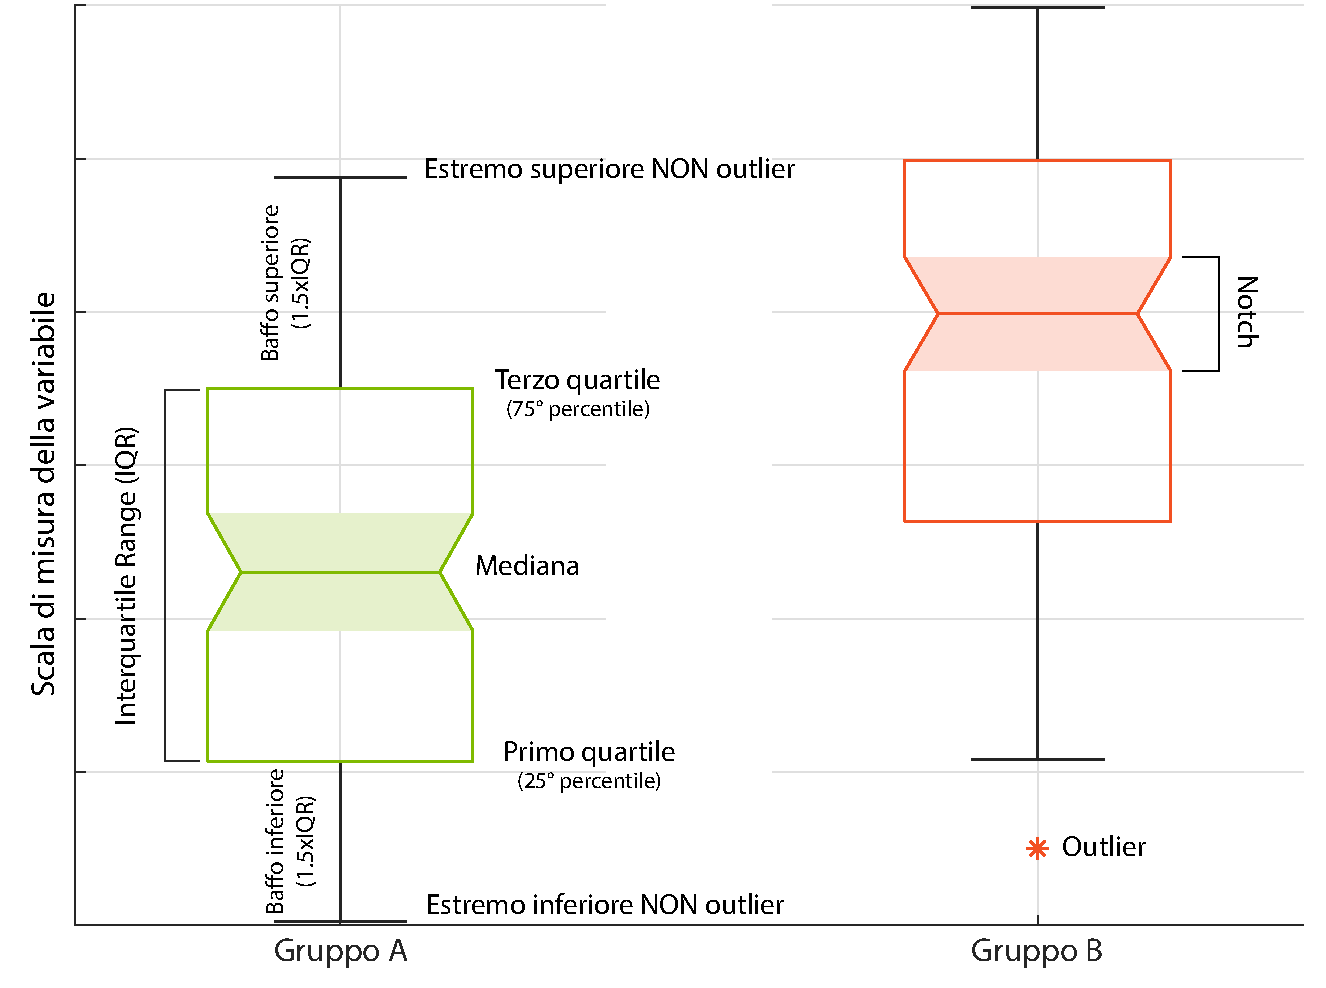
\includegraphics[width=0.9\textwidth]{Figure/esempionotch.pdf}
    \caption{Esempio di due notched boxplot, le cui mediane hanno una differenza statisticamente significativa. Dettagli nel testo.}
    \label{fig:notch}
\end{figure}

Per una visualizzazione più immediata delle inferenze statistiche sono stati costruiti anche dei \emph{notched boxplot} \cite{McGill1978}, strumenti utili al fine di graficare eventuali differenze statisticamente significative (con p--value $< \alpha$) tra mediane di gruppi diversi. Infatti, nel caso in cui i \emph{notch} di due boxplot a confronto non si sovrappongano, come nell'esempio rappresentato in figura \ref{fig:notch}, si può affermare con il livello di confidenza $(1-\alpha)$ che sussiste una differenza significativa tra le due mediane. 

Gli estremi superiore ed inferiore del notch corrispondono, per la confidenza convenzionale del 95$\%$, al valore della mediana~$\pm {1.57 \times \mathrm{IQR}}/{\sqrt{n}} $, dove $n$ è la dimensione del campione e $\mathrm{IQR}$ è l'\textsl{Interquartile Range} o lo scarto interquartile, ovvero la differenza tra il terzo ed il primo quartile \cite{McGill1978}.\\

Per garantire la completa riprodicibilità dei risultati presentati in appendice \ref{appendix:code} sono riportati tutti i codici \textsc{Matlab}\textsuperscript{\tiny\sffamily\textregistered} utilizzati per generare le figure e operare i test d'ipotesi. Alcuni dei comandi adoperati, segnalati in {\mlttfamily\color{xkcdLilac}\bfseries\itshape grassetto--corsivo--lilla}, non sono nativi del software base, ma importati dal già citato toolbox o da pacchetti esterni\footnote{In particolare, {\mlttfamily\bfseries\itshape\color{xkcdLilac}kruskalwallis()} e {\mlttfamily\bfseries\itshape\color{xkcdLilac}multcompare()} sono inclusi nello \textsc{statistics and machine learning toolbox}, mentre {\mlttfamily\bfseries\itshape\color{xkcdLilac}export\_fig()}, {\mlttfamily\bfseries\itshape\color{xkcdLilac}fig2svg()} e {\mlttfamily\bfseries\itshape\color{xkcdLilac}hex2rgb()} sono resi disponibili, sotto licenza \emph{open--source}, dalla multilibreria \textsc{the matverse}: \url{https://github.com/bellomia/MATVERSE} }. In altri casi ancora si tratta di funzioni speciali definite appositamente dall'autrice: queste ultime sono integralmente riportate in sezione \ref{code:subroutines}.




